% Figure 2.4 (Session 2): the uniform and the dimerized Heisenberg chain, the triplet excitation
% and the induced moments from a pinned end.
% The image is rendered by figures/blender/s2_4_dimerized.py; the coordinates of the labels
% come from figures/blender/out/dimerized_anchors.tex. Compile with:
%   pdflatex dimerized.tex ; result moves to ../quantum_magnetism/dimerized.pdf
\documentclass[11pt,tikz,border=0pt]{standalone}
\usepackage{amsmath,amssymb,graphicx,braket}
\usepackage{xcolor}
\definecolor{coursedark}{HTML}{1B2A4A}
\definecolor{costamber}{HTML}{B8620A}
\newlength{\figw}\setlength{\figw}{16.19cm}   % the text width of the notes (letter, 2.7 cm margins), so labels print at size

\begin{document}
\begin{tikzpicture}[lbl/.style={font=\small, text=coursedark}]
  \node[anchor=south west, inner sep=0pt] at (0,0)
    {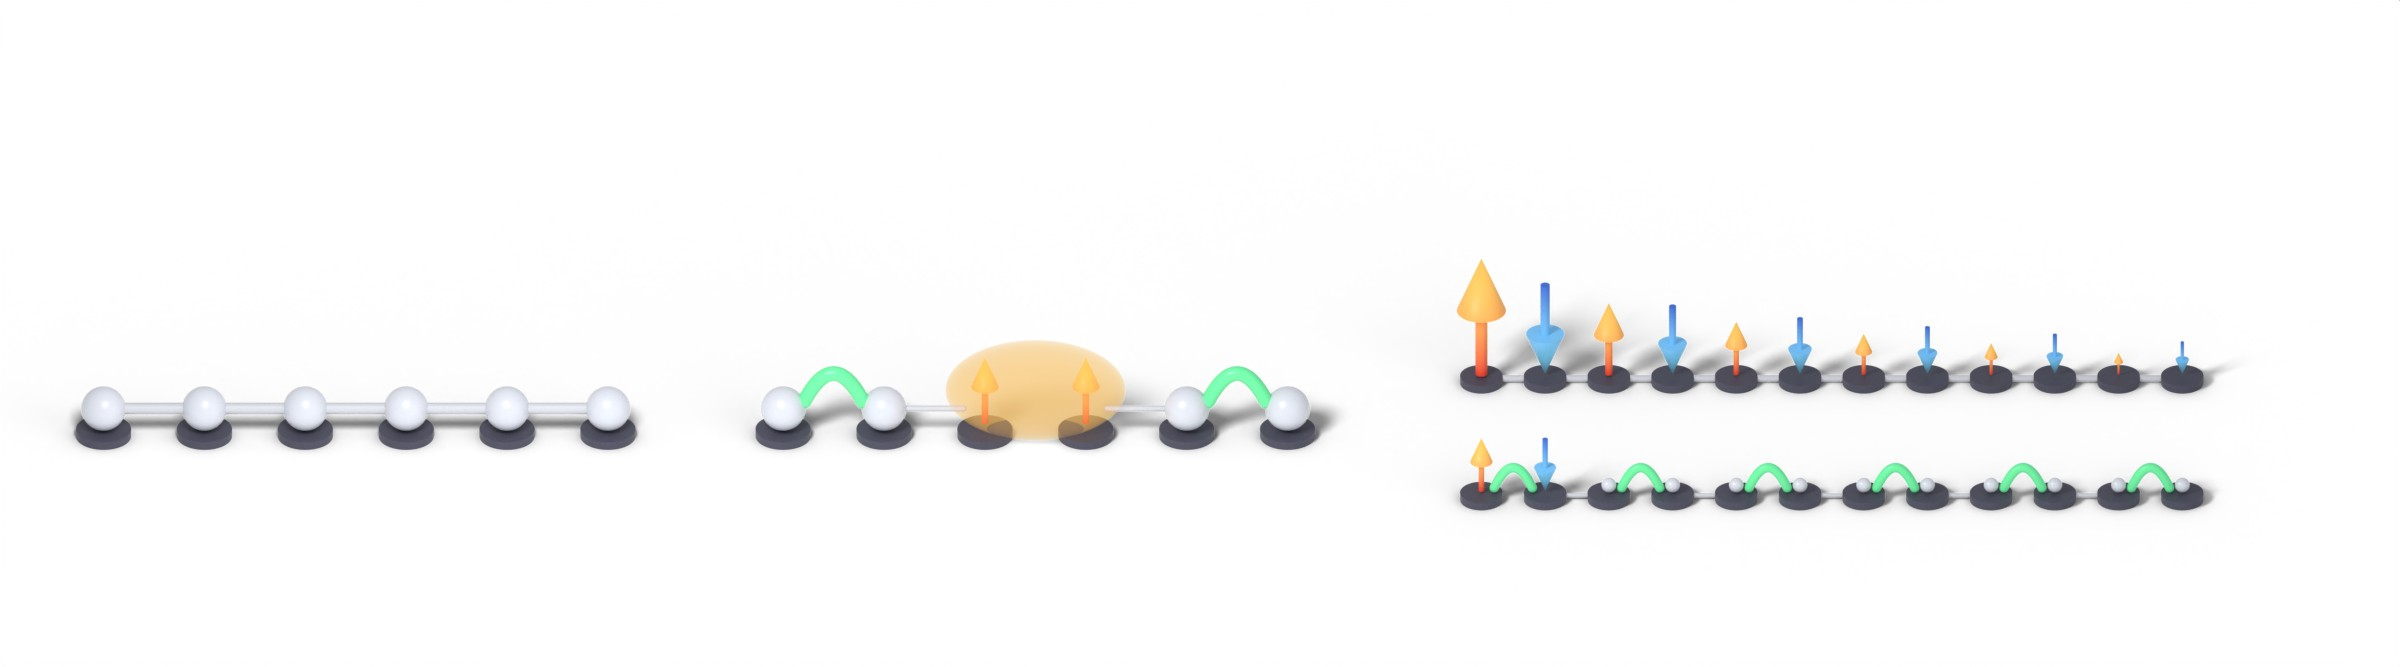
\includegraphics[width=\figw]{../blender/out/dimerized.jpg}};
  %% written by figlib.py; x and y in units of the image width
\coordinate (a) at (0.0199\figw,0.1882\figw);
\coordinate (labA) at (0.1482\figw,0.0763\figw);
\coordinate (T) at (0.4314\figw,0.1395\figw);
\coordinate (b) at (0.3031\figw,0.1882\figw);
\coordinate (labB) at (0.4314\figw,0.0763\figw);
\coordinate (h_cu) at (0.6040\figw,0.1375\figw);
\coordinate (end_cu) at (0.9226\figw,0.1298\figw);
\coordinate (h_cd) at (0.6040\figw,0.0888\figw);
\coordinate (end_cd) at (0.9226\figw,0.0812\figw);
\coordinate (c) at (0.5774\figw,0.2103\figw);
\coordinate (labC) at (0.7633\figw,0.0498\figw);

  \node[lbl, font=\normalsize, anchor=west] at (a) {(a)};
  \node[lbl, font=\normalsize, anchor=west] at (b) {(b)};
  \node[lbl, font=\normalsize, anchor=west] at (c) {(c)};
  \node[lbl, anchor=north] at (labA) {uniform, every bond $J$};
  \node[lbl, anchor=north] at (labB) {dimerized, $J(1\pm\delta)$};
  \node[lbl, text=costamber, anchor=south] at (T) {triplet, $\approx J(1+\delta)$};
  \node[lbl, anchor=east] at (h_cu) {$h$};
  \node[lbl, anchor=east] at (h_cd) {$h$};
  \node[lbl, anchor=west] at (end_cu) {$\delta=0$};
  \node[lbl, anchor=west] at (end_cd) {$\delta=0.5$};
  \node[lbl, anchor=north] at (labC) {induced moments $\langle S^z_j\rangle$};
\end{tikzpicture}
\end{document}
